\documentclass[dvipsnames,hyperref={pdfpagelabels=false}]{beamer}
% beamer already loads hyperref; do NOT load \usepackage{hyperref} again.

\usepackage{ragged2e} % 文字向兩邊對齊
\renewcommand{\raggedright}{\leftskip=0pt \rightskip=0pt plus 0cm}

\usepackage{listings}
\usepackage{lmodern}
\usepackage{fontspec}
\usepackage{xeCJK}
\setCJKmainfont{Noto Sans CJK TC}
\setCJKsansfont{Noto Sans CJK TC}
\setCJKmonofont{Noto Sans Mono CJK TC}

\usepackage[english]{babel}
\usepackage{amsmath,amssymb,amsfonts,amsthm}

% hyperref settings (since beamer already loads hyperref)
\hypersetup{
  colorlinks=true,
  urlcolor=blue,
  citecolor=blue,
  pdfborder={0 0 0}
}

\usepackage{accsupp}% http://ctan.org/pkg/accsupp
\newcommand{\emptyaccsupp}[1]{\BeginAccSupp{ActualText={}}#1\EndAccSupp{}}

\usepackage{tikz}
\usetikzlibrary{arrows,decorations.pathmorphing,backgrounds,fit,positioning,shapes.symbols,chains}
\usetikzlibrary{tikzmark}

\usepackage{booktabs}
\usepackage{threeparttable}
\usepackage{colortbl}
\usepackage{xcolor}

\newcommand{\indep}{\perp\!\!\!\perp}
\newcommand{\nindep}{\not\!\perp\!\!\!\perp}

\beamertemplatefootpagenumber


\title[]
{Guidelines for Oral Exam}

\author
{Prof. Tzu-Ting Yang}

\institute{Institute of Economics, Academia Sinica}

\date{\today}


\usetheme{CambridgeUS}
\setbeamertemplate{footline}{%
	\hfill\usebeamercolor[fg]{page number in head/foot}%
	\usebeamerfont{page number in head/foot}%
	\insertframenumber\,/\,\inserttotalframenumber\hspace{1em}\vspace{2pt}%
}

\beamersetuncovermixins{\opaqueness<1>{25}}{\opaqueness<2->{15}}

\begin{document}

\begin{frame}{}
	\titlepage
\end{frame}


%-------------------------------------------------------------
\begin{frame}{Oral Exam: Overview}

\begin{itemize}
	\item The oral exam serves as a \textbf{discussion of your term paper}
	\vspace{0.3cm}

	\item It tests two things:
	\vspace{0.2cm}
	\begin{itemize}
		\item[(1)] Whether you truly understand the \textbf{empirical method} you used in your term paper
		\vspace{0.2cm}
		\item[(2)] Whether you understand the \textbf{programming commands} you used in homework (R or Stata)
	\end{itemize}
	\vspace{0.3cm}

	\item There will be \textbf{at least two questions}, one for each area above
	\vspace{0.3cm}

	\item Follow-up questions may be asked depending on your answers
\end{itemize}

\end{frame}


%-------------------------------------------------------------
\begin{frame}{Question 1: Empirical Method}

\begin{block}{What is tested}
	You must be able to, on the spot:
	\begin{itemize}
		\vspace{0.1cm}
		\item \textbf{Write out the mathematical formula} of your empirical method\\
		      (e.g., regression equation, identification assumption, estimator)
		\vspace{0.1cm}
		\item \textbf{Explain what each symbol means} and the intuition behind the method
		\vspace{0.1cm}
		\item Answer \textbf{follow-up questions} about the method
	\end{itemize}
\end{block}

\vspace{0.3cm}

\begin{exampleblock}{How to prepare}
	\begin{itemize}
		\item Re-read the empirical strategy section of your term paper
		\vspace{0.1cm}
		\item Make sure you can explain your method \textbf{without looking at slides}
		\vspace{0.1cm}
		\item Think about: what is the \textbf{key identifying assumption}?\\
		      What goes wrong if it fails?
	\end{itemize}
\end{exampleblock}

\end{frame}


%-------------------------------------------------------------
\begin{frame}{Question 1: Examples}

\vspace{0.1cm}
\small
Sample questions depending on the method in your term paper:

\vspace{0.3cm}
\begin{tabular}{p{0.28\textwidth} p{0.64\textwidth}}
\toprule
\textbf{Method} & \textbf{Possible question} \\
\midrule
OLS / Regression &
Write out your regression equation and explain what $\hat{\beta}$ means. \\[6pt]
Difference-in-Differences &
Write the DiD estimator. What does the parallel trends assumption say? \\[6pt]
Instrumental Variables &
Write the first-stage equation. Why is your instrument valid? \\[6pt]
Regression Discontinuity &
Explain the RDD identification strategy. What does the estimate capture? \\[6pt]
Matching / PSM &
Define the propensity score. What is the intuition behind matching? \\
\bottomrule
\end{tabular}

\end{frame}


%-------------------------------------------------------------
\begin{frame}{Question 2: Programming Code}

\begin{block}{What is tested}
	Based on the language you used in homework (\textbf{R} or \textbf{Stata}):
	\begin{itemize}
		\vspace{0.1cm}
		\item Explain what a piece of \textbf{code does} --- what each command or option means
		\vspace{0.1cm}
		\item \textbf{Interpret the output}: what do the numbers tell you?
		\vspace{0.1cm}
		\item If a parameter is changed, \textbf{how would the result differ}?
	\end{itemize}
\end{block}

\vspace{0.3cm}

\begin{exampleblock}{How to prepare}
	\begin{itemize}
		\item Re-run your homework code and make sure you understand every line
		\vspace{0.1cm}
		\item You do not need to memorise syntax, but you must understand \textbf{what each command does}
		\vspace{0.1cm}
		\item Key skill: given a snippet of code, \textbf{connect it to the underlying statistical concept}
	\end{itemize}
\end{exampleblock}

\end{frame}


%-------------------------------------------------------------
\begin{frame}{Question 2: Examples}

\vspace{0.1cm}
\small
Sample code questions:

\vspace{0.25cm}
\begin{block}{R example}
\texttt{feols(y \textasciitilde{} x1 + x2 | id + year, data = df, cluster = \textasciitilde{}id)}
\begin{itemize}
	\item What does \texttt{| id + year} do? Why do we include fixed effects?
	\item What is the role of \texttt{cluster = \textasciitilde{}id}? What happens if you omit it?
\end{itemize}
\end{block}

\vspace{0.2cm}
\begin{block}{Stata example}
\texttt{ivregress 2sls y x1 (x2 = z), robust first}
\begin{itemize}
	\item What does \texttt{(x2 = z)} specify? What role does \texttt{z} play?
	\item What does the \texttt{first} option display? How do you assess instrument strength?
\end{itemize}
\end{block}

\end{frame}


%-------------------------------------------------------------
\begin{frame}{Summary}

\begin{center}
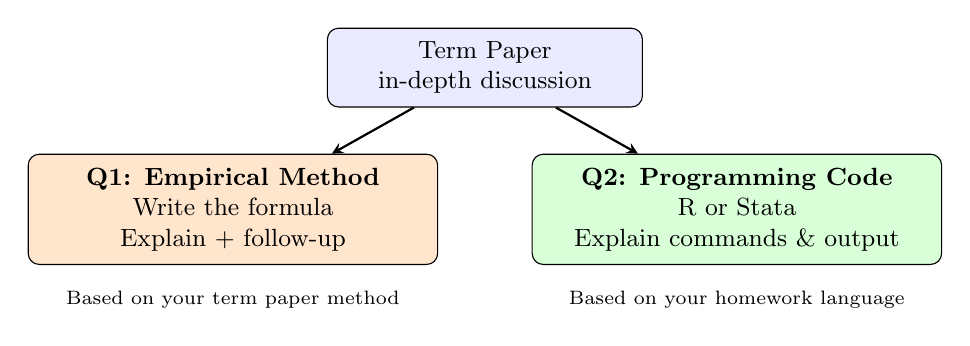
\begin{tikzpicture}[
  box/.style={rectangle, draw, rounded corners, align=center,
              minimum width=4.0cm, minimum height=1.0cm,
              font=\small, fill=blue!8},
  qbox/.style={rectangle, draw, rounded corners, align=center,
               minimum width=5.2cm, minimum height=1.4cm,
               font=\small},
  arrow/.style={->, >=stealth, thick}
]

\node[box] (tp) at (0, 2.2) {Term Paper\\in-depth discussion};

\node[qbox, fill=orange!20] (q1) at (-3.2, 0.4)
  {\textbf{Q1: Empirical Method}\\Write the formula\\Explain + follow-up};

\node[qbox, fill=green!15] (q2) at (3.2, 0.4)
  {\textbf{Q2: Programming Code}\\R or Stata\\Explain commands \& output};

\draw[arrow] (tp) -- (q1);
\draw[arrow] (tp) -- (q2);

\node[font=\scriptsize, align=center] at (-3.2, -0.75)
  {Based on your term paper method};
\node[font=\scriptsize, align=center] at (3.2, -0.75)
  {Based on your homework language};

\end{tikzpicture}
\end{center}

\vspace{0.1cm}
\begin{center}
\fbox{\parbox{0.85\textwidth}{\centering
	The oral exam is not meant to trick you.\\
	It is a chance to show that you understand what you did\\
	in your term paper and homework.
}}
\end{center}

\end{frame}


\end{document}
